\section{Components}
The~game server is divided into separate components. Many instances of a~component can run at~the~same time. Component, and even instances, can be distributed among many machines; this feature renders the~whole server easily scalable. Refer to Figure \ref{fig:components} for a~component diagram.

\begin{figure}[h]	
	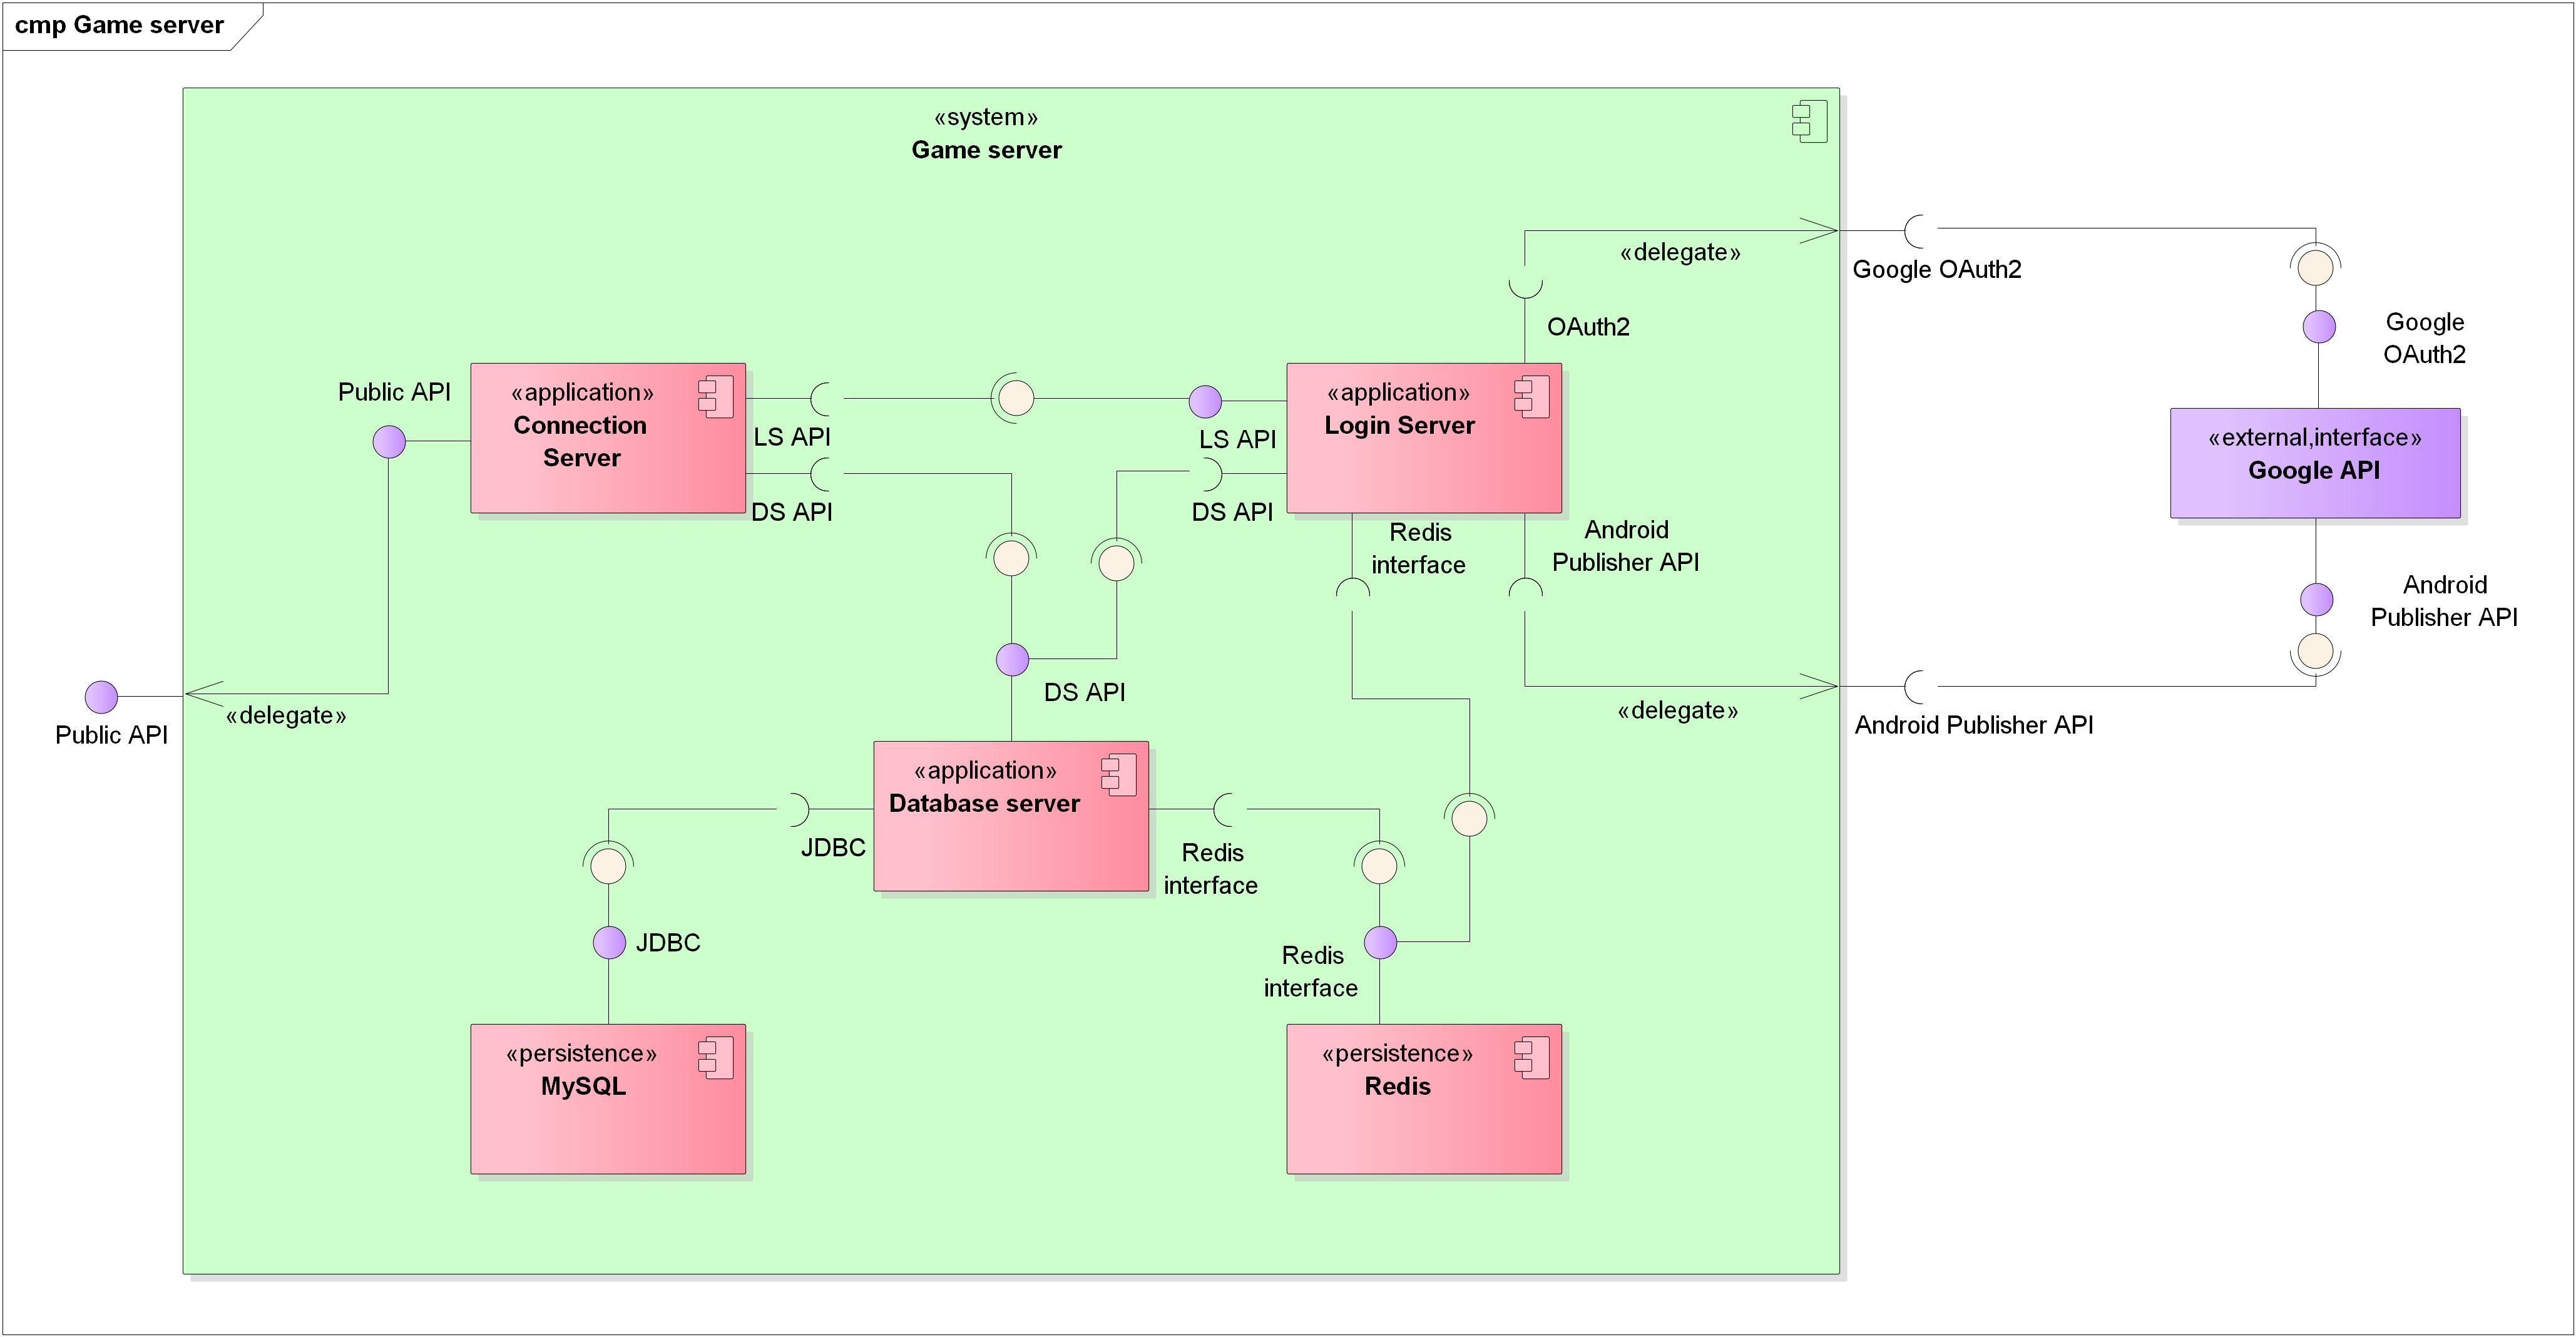
\includegraphics[width=\textwidth]{figures/Components}
	\centering			
	\caption{Component diagram of the~game server}
	\label{fig:components}
\end{figure}

	\subsection{Connection server}
	This is the~public entry point and the~only component exposed to clients. Reducing the~number of publicly accessible components increases security of the~server. CS handles all incoming traffic and delegates work to other components. 
	
	\subsection{Login server}
	The~main responsibility of the~LS is to handle user authentication and authorization. It connects to Redis where users' access codes are stored. The~LS is also used for in-app purchase verification. The~component is connected to Google API.
	
	\subsection{Database server}
	The~most important component is Database server. Most of the~game logic happens here. Since the~DS is responsible for data~persistence, it is connected to MySQL and Redis.

\section{Activities}
	\subsection{Authentication}
	Authentication process is visualized in Figure \ref{fig:adauth}.
	
	\begin{figure}[h]	
		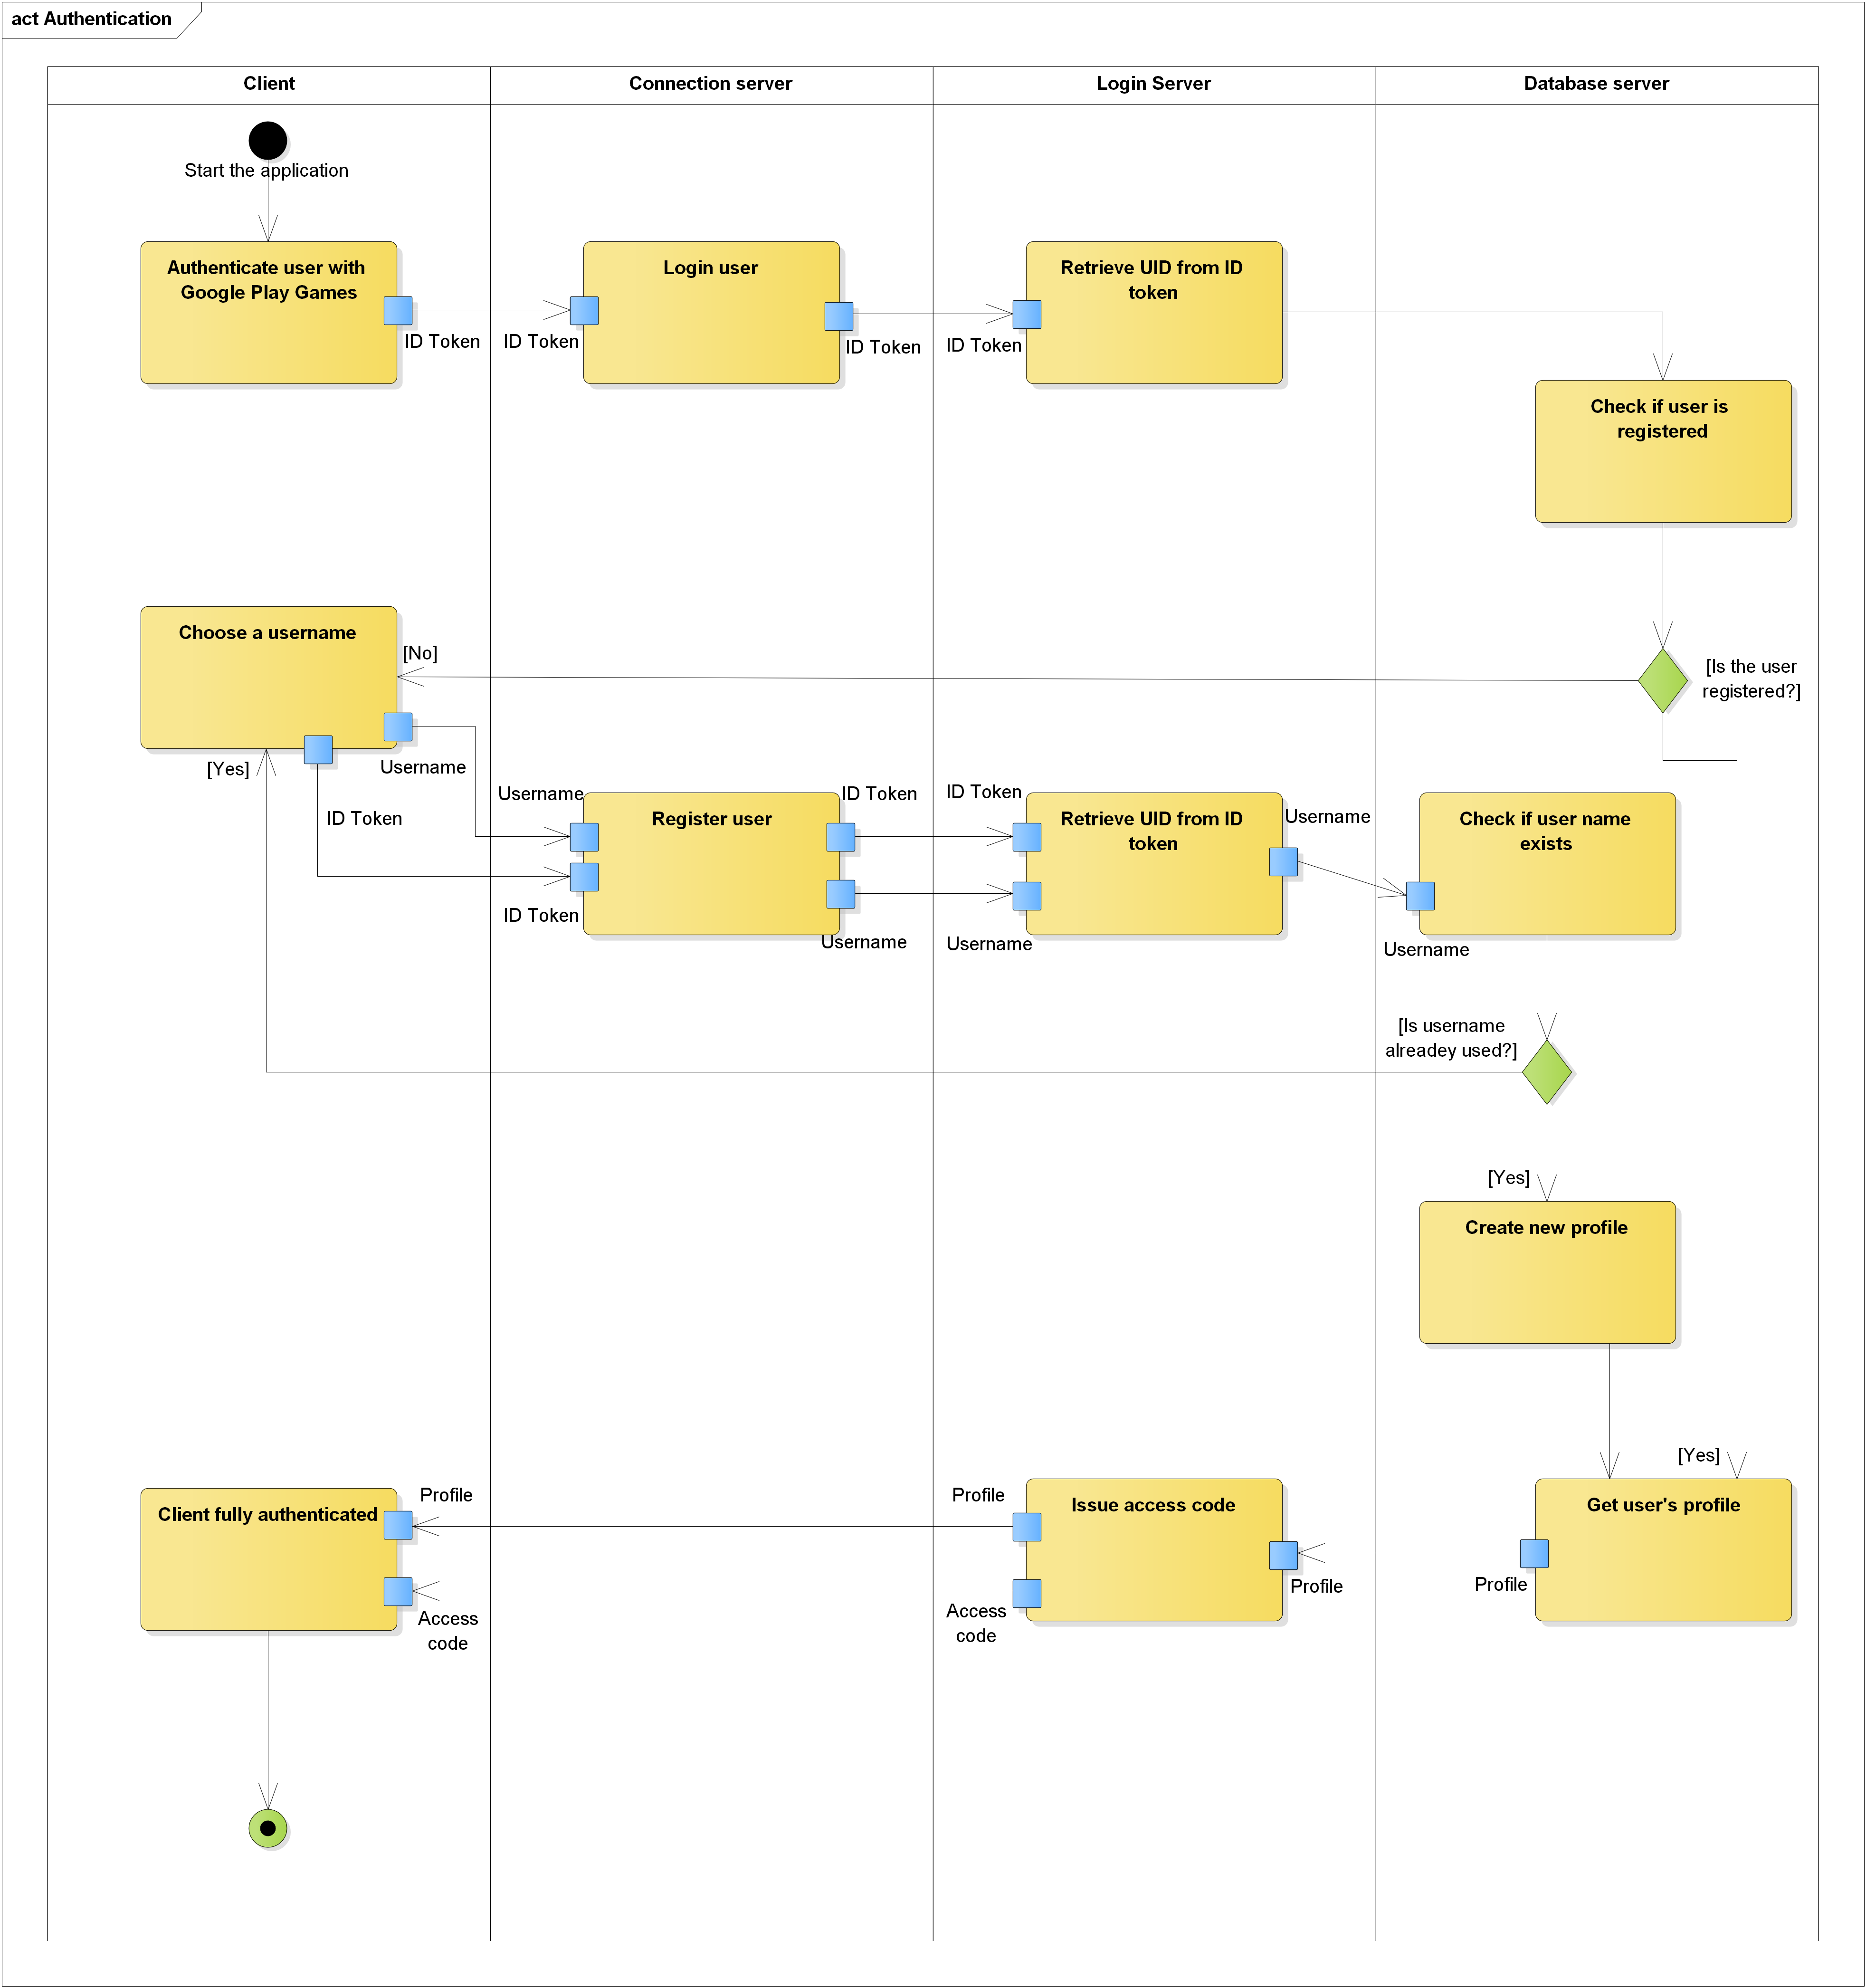
\includegraphics[width=\textwidth]{figures/AD_Authentication}
		\centering			
		\caption{Activity diagram of the~authentication process}
		\label{fig:adauth}
	\end{figure}

		\subsubsection{Access code}
		A~client is identified by his access code during a~session. The~code is random and unique. It is generated each time the~client finishes login process; the~old code,  previously issued to the~user, is invalidated.
		
		\subsubsection{Registration}
		Every user must register an account to gain access to the~game. The~user is asked to choose a~unique username. If the~username is already taken, the~whole registration process has to be repeated. LS retrieves user's UID and his e-mail address and passes the~information to the~DS, which then creates and initializes a~new user profile. Client is issued an access code and the~authentication process is completed.
		
		\subsubsection{Login}
		A~registered user can simply login using only his ID Token, which is provided to client during login process by Google Play Games. LS exchanges the~token for UID which is then used to retrieve user's profile. Client is issued an access code and the~authentication process is completed.
	
	\subsection{Killing a~monster}
	A user decides to fight a \textit{monster}. In this prototype, the client iteratively deals damage to the user and the \textit{monster}. The damage is calculated as \textit{attackDamage} attribute multiplied by a random value 0.5-1.5. If \textit{health} of the \textit{monster} drops to below zero before the user's one does, the \textit{monster} is killed. Server is notified of the result and rewards the user with \textit{gold} and \textit{experience}. The kill is logged, the \textit{monster} is removed from the game map and the client is provided with a one-time \textit{killConfirmationCode} which allows him to collect loot from the \textit{monster}.
		
	\subsection{Killing a~user}
	If user's \textit{health} drops to or below before the \textit{monster}'s one, the user dies. Client notifies the server of user's death. His \textit{health} is fully restored and he's punished with \textit{deathPenalty} which is deducted from his gold:  \[ deathPenalty = 200 + 100 * (userLevel - 1) \]
	
	\subsection{Collecting loot after kill}
	User is presented with an option to collect loot from a \textit{monster} he killed. Clients sends a \textit{killConfirmationCode} along with a list of items, he wants to collect, to the server. DS consumes the \textit{killConfirmationCode} and adds the selected items to user's inventory. Client then receives the updated inventory.
	
	\subsection{Buying an item}
	Client shows its user a \textit{shop} and lets him choose what item he wants to buy. The selected item is sent to the server. DS verifies the item is in the specified \textit{shop}. Price of the item is then deducted from user's account and the item is added to his inventory. If the user does not have enough \textit{gold}, the purchase is rejected and an error message is returned. Otherwise, client receives updated user's inventory.
	
	\subsection{Equipping an item}
	User selects a \textit{slot} and an appropriate item from his inventory. The client sends the item along with the slot to the server. DS checks if the item-slot pair is correct and assigns the item to the \textit{slot}. The successful result is then confirmed to the client.
	
	\subsection{Using an item}
	User selects a usable item from his inventory. Client sends the selected item to the server. DS decides what the item does by looking at attributes \textit{addHealth}, \textit{addExperience}, and \textit{addGold}. Based o the values set for the item, health, experience, and/or gold is added to user's account. The updated profile is then sent back to the client.
		
	\subsection{Purchasing in-app product}
	In-app purchases are handled on client which performs the transaction using a Google service. The prototype currently supports only buying \textit{gold}. If the transaction is successful, client sends a Google's \textit{Purchase token} to the server. LS verifies the status of the purchase using \textbf{Android Publisher API} \cite{androidpublisher} and adds the \textit{gold} to user's account. The purchase is then confirmed to the client.

	\subsection{Retrieving nearby game objects}
	Client visualizes nearby \textit{game objects} on the map. Since the user moves, the client frequently retrieves new \textit{game objects} based on the actual location, making high demands on the speed of the retrieval process.
	
	\begin{figure}[h]	
		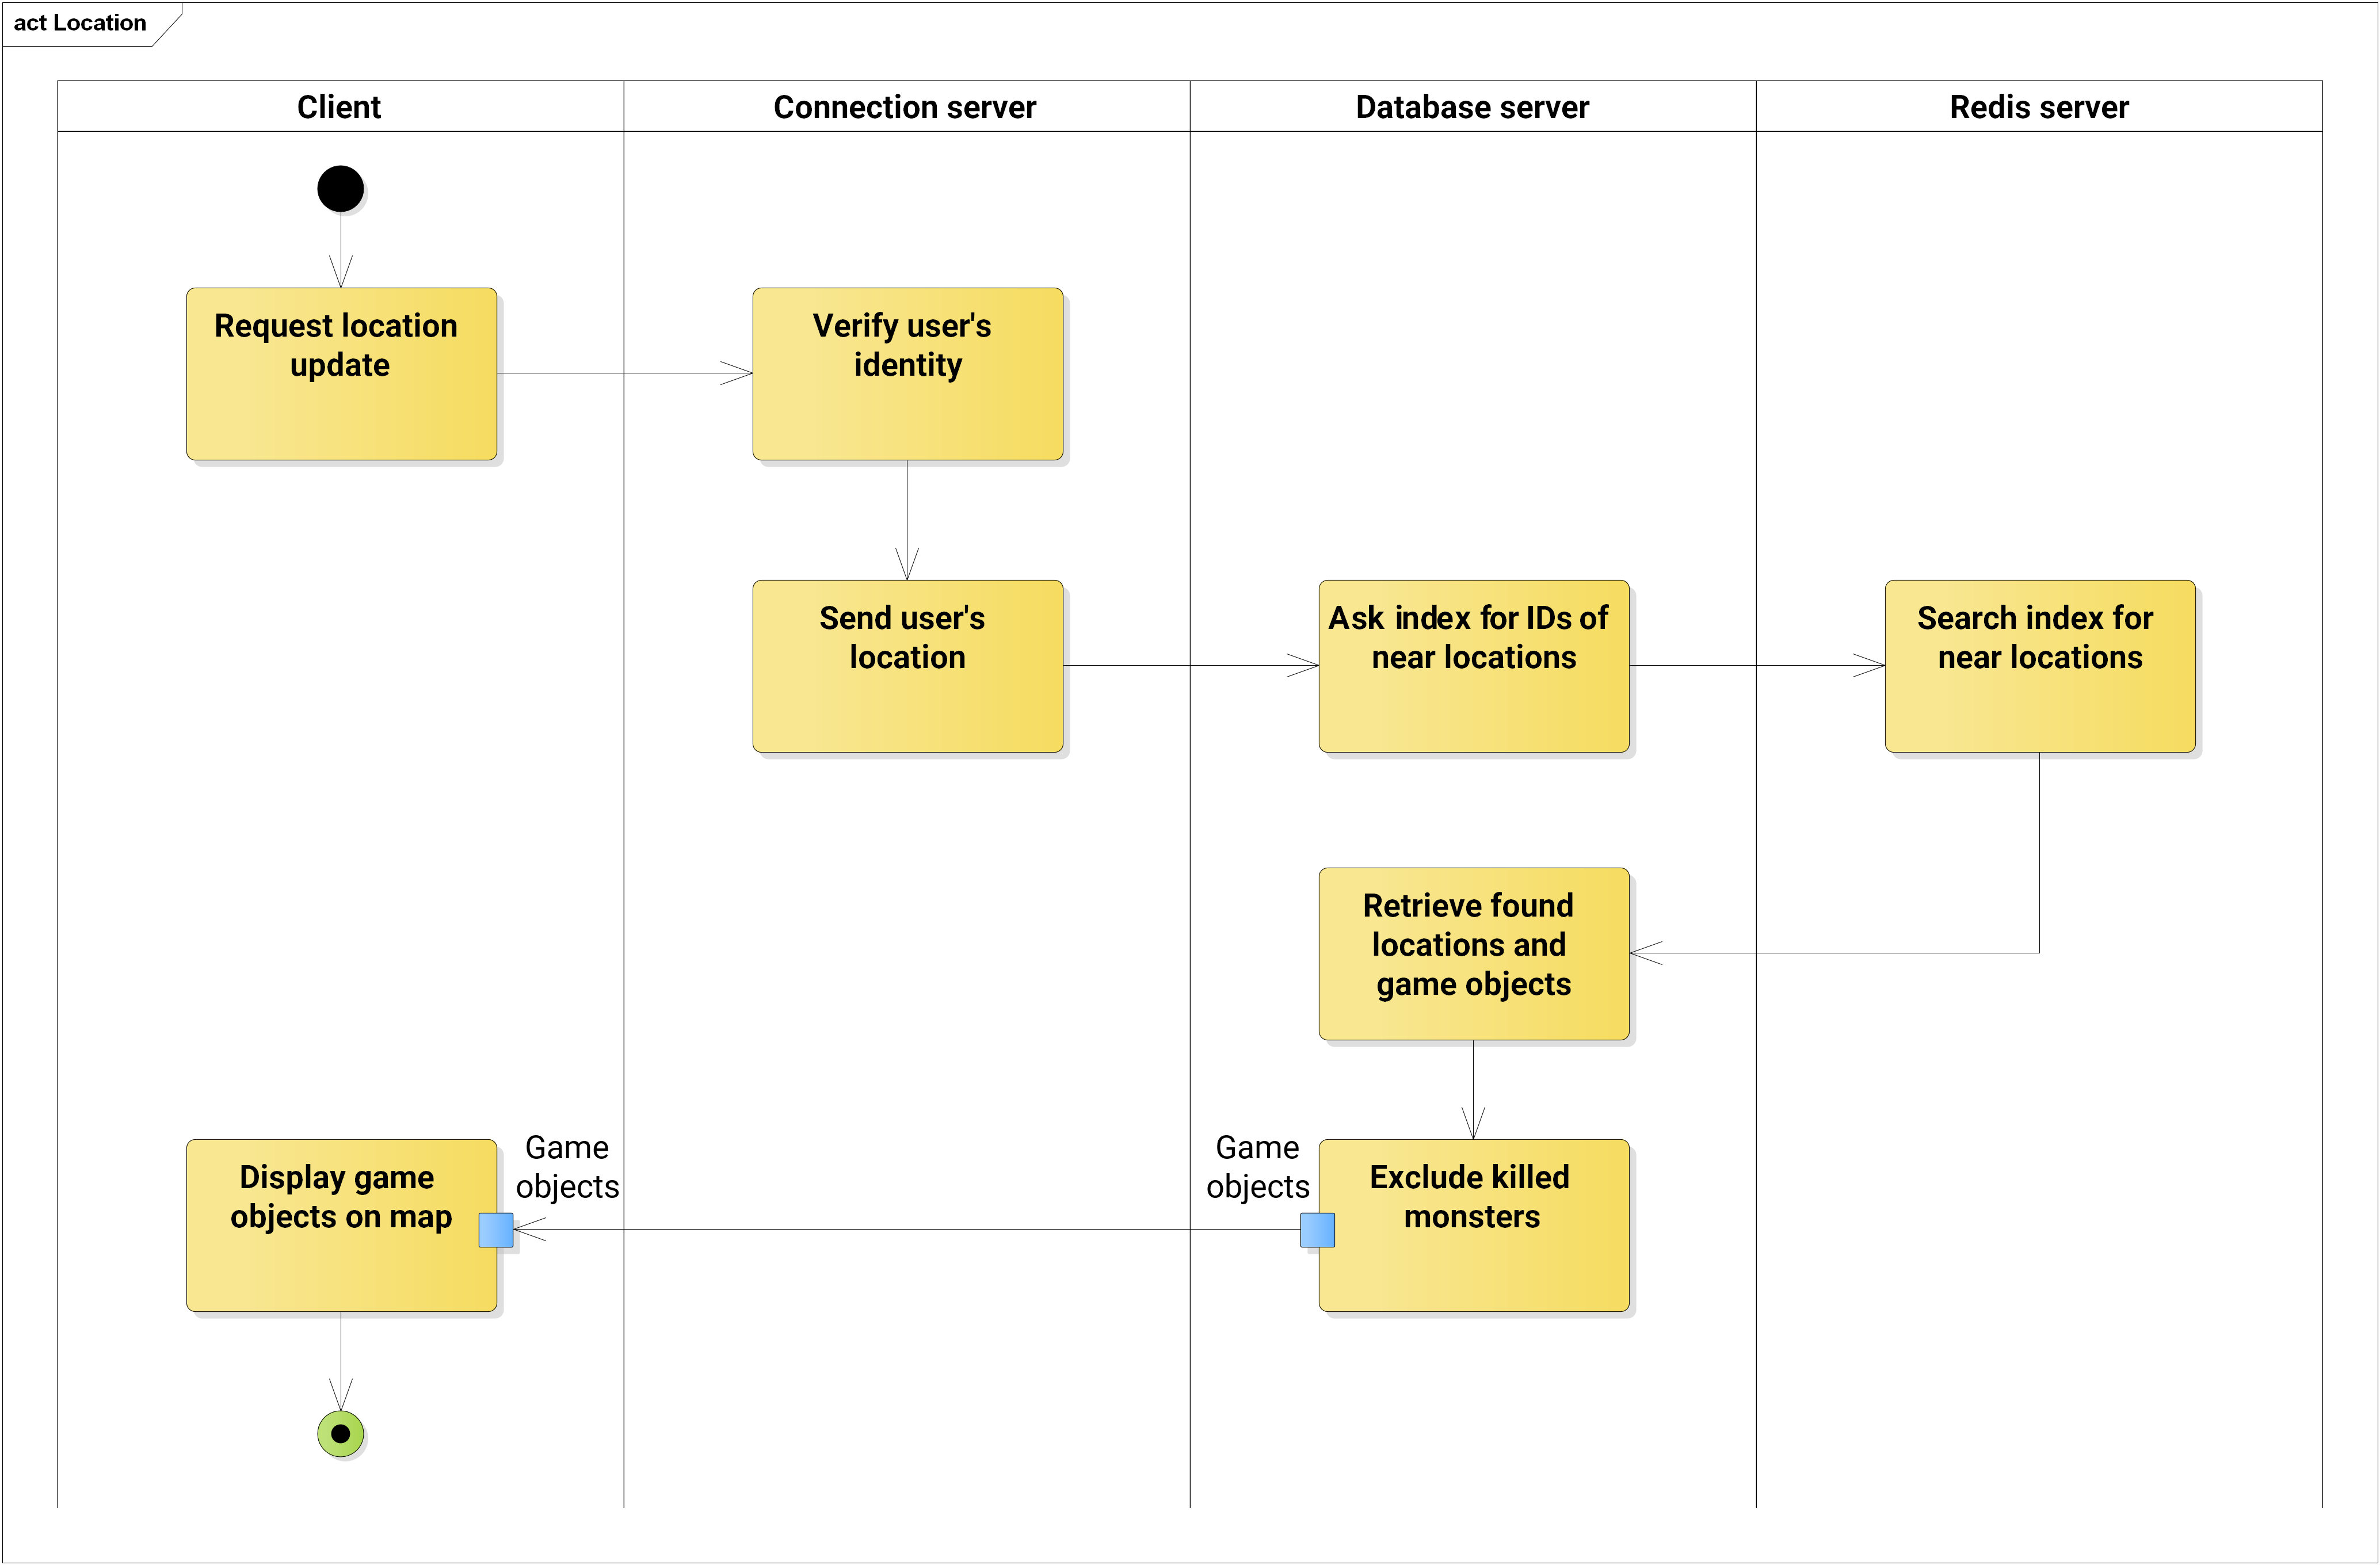
\includegraphics[width=\textwidth]{figures/AD_Location}
		\centering			
		\caption{Activity diagram of how the~server provides nearby game objects}
		\label{fig:adlocation}
	\end{figure} 
	
	Client sends its coordinates to the server. DS queries Redis which contains an index of all available \textit{locations}. The index responds with IDs of \textit{locations} in 200 m radius from the provided coordinates. The \textit{locations} and their assigned \textit{game objects} are then retrieved from the database. Server excludes already killed \textit{monsters}. The list of \textit{locations} and their \textit{game objects} is sent to the client which presents them on the map. See an activity diagram of the described process in Figure~\ref{fig:adlocation}.		

\section{Database Model}
	The database was designed to comply with the requirements specified in section \ref{section:requirements}. The entire database model is shown in Figure \ref{fig:dbmodel}. In the following text, I will describe important tables.	
	
	\begin{figure}[h]	
		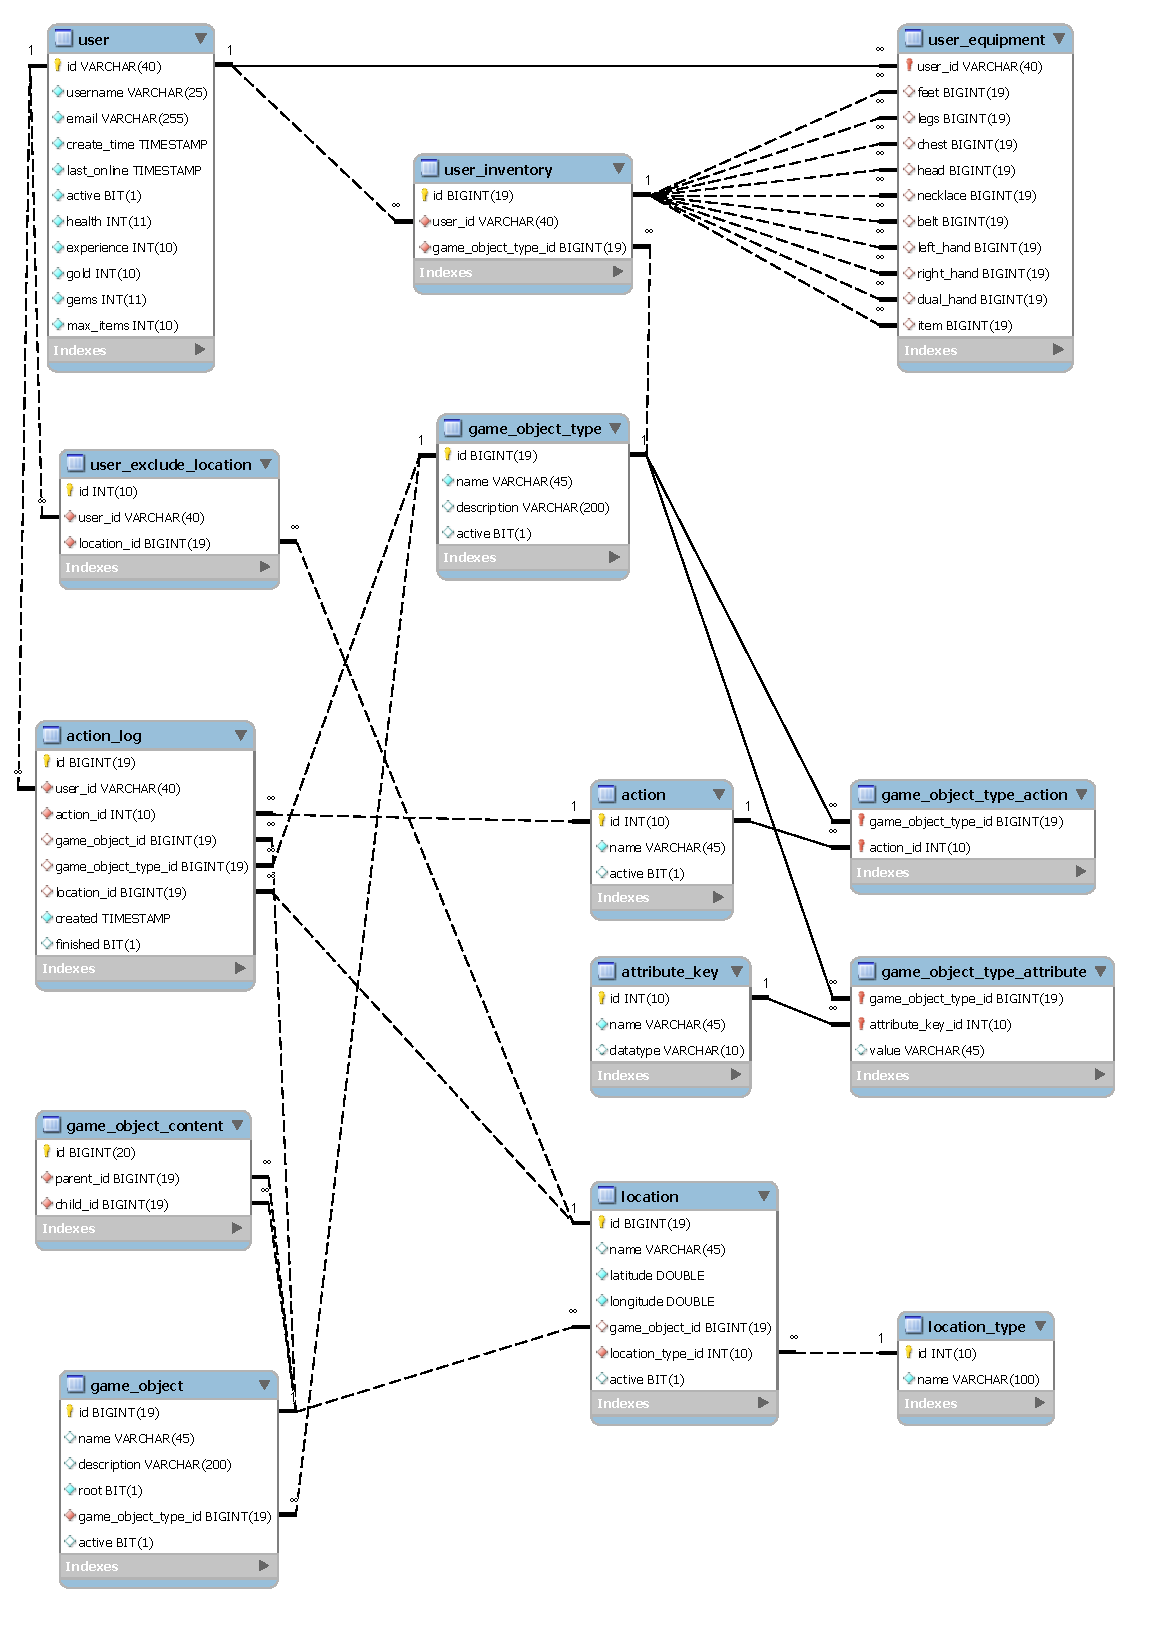
\includegraphics[width=\textwidth]{figures/DatabaseModel}
		\centering
		\caption{Database model}
		\label{fig:dbmodel}	
	\end{figure}
	
	\begin{description}
		\item[user] User's profile. It contains \textit{e-mail}, \textit{UID}, and \textit{username}. Quality attributes of the profile are also stored here - current \textit{health}, \textit{experience}, and \textit{gold}.
		
		\item[user\_inventory] Items a user own. 
		
		\item[user\_equipment] Information about what items a user has equipped. Is in 1:1 relationship with \textit{user}. Each column represents an equipment \textit{slot}. When an item is equipped, the item's entry from \textit{user\_inventory} to its \textit{slot}.
		
		\item[game\_object\_type] A "recipe" for every object in the game. Name and description of an object is stored here. The \textit{game\_object\_type} has linked attributes and actions.
	
		\item[action] Defines all allowed \textit{actions}. Each \textit{game object type} implements their subset.
		
		\item[game\_object\_type\_attribute] Defines all \textit{attributes} of a \textit{game object}. The attribute is identified by its \textit{name} and can have a \textit{value}.
	
		\item[game\_object] An implementation of \textit{game object type} which can be assigned to a \textit{location}.
	
		\item[game\_object\_content] Inventory of a \textit{game object}
	
		\item[location] Predefined real-world locations. Each one must have \textit{latitude} and \textit{longitude} defined; \textit{location} can have a \textit{game object} assigned. 
	
		\item[action\_log] Log of user's actions. In prototype, it is used only for kills to allow collecting loot.

		\item[user\_exclude\_location] Locations at which a user killed a monster. The table is periodically flushed. 
		
	\end{description}

\section{Administration}
The \textit{Database server} supports several API endpoints through which authorized administrators can manage the game data. The \textit{Admin} section is protected using \textbf{HTTP Basic Authentication} and thus the administrator has to know a valid username-password combination. For prototyping purposes, I've decided to provide only basic functionality for the administration.

	\subsection{Game object type management}
	Administrator can create new \textit{game object types} by sending a POST request to the endpoint \mbox{\textit{/admin/gameObjectType}}. A unique \textit{name} has to be specified for the new type. Optionally, the type can include a \textit{description}, a set of allowed \textit{actions} and \textit{attributes}.
	
	Existing \textit{game object types} can be updated. It is possible to change all their properties like \textit{name} and \textit{description}. Administrator can also add new \textit{attributes} and \textit{actions}. This is done using PUT request to the endpoint \mbox{\textit{/admin/gameObjectType}}
		
	All existing \textit{game object types} can be retrieved along with their \textit{actions} and \textit{attributes} by sending a GET request to the endpoint \mbox{\textit{/admin/gameObjectType}}
	
	\subsection{Game object management}
	Administrator can create new \textit{game objects} by sending a POST request to the endpoint \mbox{\textit{/admin/gameObject}}. \textit{Game object type} have to be specified for the new \textit{game object}. Optionally, the new object can have a set of children which can be later updated by calling PUT \mbox{\textit{/admin/gameObject}}.
	
	All existing \textit{game objects} can be retrieved along with their children by sending a GET request to the endpoint \mbox{\textit{/admin/gameObject}}
	
	\subsection{Location import}
	New locations can be imported from a file in OSM XML \cite{osmxml}. Administrator can do so be sending a POST request to \mbox{\textit{/admin/importLocations}}. The file is parsed for latitude and longitude data nad the new locations are inserted into the database.
	
	\subsection{Game object to a location assignment}
	A location serves no purpose without a\textit{game object} assigned to it. This can be achieved by using PUT endpoint \mbox{\textit{/admin/assignGameObjectToLocation}}.
	
	\subsection{Cache clearing}
	During the development process, developers might need to change game data by accessing the database directly. Since Hibernate won't be aware of such changes, its cache must be cleared via DELETE endpoint\mbox{\textit{/admin/clearCache}}.

\section{Calculations}
	\subsection{User's level}
	\[ level = \left\lfloor{\left(\frac{xp}{1024}\right)^{0.62} + 1}\right\rfloor, \]
	where $xp$ is user's experience.
	\subsection{Maximum health}
	Player's cannot exceed a certain value which linearly scales with his level.
	\[ maxHealth = 200 + 50 * (userLevel - 1) \]
	
	\subsection{Death penalty}
	A player is punished by losing gold when he dies. The total amount of the lost gold scales with user's level.
	\[ deathPenalty = 200 + 100 * (userLevel - 1) \]

\section{Public API}
Even though every component has its own API, only the~Connection Server API is available to clients. HTTP methods correspond to REST principles.

The~public API for the~prototype has been specified in cooperation with my colleague Tomáš Zahálka. Below are shortly described selected endpoints. For the~full list of publicly available API enpoints, please refer to Appendix~\ref{appendix:api}. The~mentioned appendix also contains description of API provided by LS and DS. 	

\subsection{GET /login}

The~Login endpoint verifies the~Google ID token and generates an~\textit{Access Code} for identification. When successfully authenticated, the~user's profile and the~\textit{Access Code} are returned.

\subsubsection*{Parameters}

\begin{description}

	\item[token] the~\textit{Google ID token}

\end{description}

\subsubsection*{Response}

\begin{description}

	\item[200] Successfully logged in, player's profile and the~\textit{Access Code} are returned.

	\item[403] Invalid token.

	\item[404] User not found, registration needed.

\end{description}

\subsection{POST /purchase}

The~Purchase endpoint offers support for in-app purchases. The~purchase is verified and then assigned to the~player. To be accepted, it cannot be cancelled or consumed.

\subsubsection*{Parameters}

\begin{description}

	\item[accessCode] the~\textit{Access Code}

	\item[productId] the~id of the~product to buy

	\item[token] the~purchase token

\end{description}

\subsubsection*{Response}

\begin{description}

	\item[200] Player's profile.

	\item[400] Invalid data.

	\item[403] Invalid \textit{Access Code} or the~purchase is not valid.

	\item[404] User not found, registration needed.

	\item[500] Unexpected error.

\end{description}

\subsection{GET /location}

This retrieves all nearby locations in a~200~m radius from the~provided coordinates. The~locations are returned along with their associated objects.

\subsubsection*{Parameters}

\begin{description}

	\item[lat] the~latitude

	\item[lon] the~longitude

	\item[accessCode] the~\textit{Access Code}

\end{description}

\subsubsection*{Response}

\begin{description}

	\item[200] List of nearby locations with game objects assigned to them.

	\item[500] Unexpected error.

\end{description}

\subsection{POST /action/kill}

The~kill action is performed on the~selected object and location. The~location is temporarily excluded from future requests to /location. The~player's health is updated, experience and gold are added. It returns a~\textit{killConfirmedCode} which is needed to perform the~collect action.

\subsubsection*{Parameters}

\begin{description}

	\item[accessCode] the~\textit{Access Code}

	\item[locationid] the~id of the~location

	\item[gameObjectId] the~id of the~game object

	\item[health] the~new player's health

\end{description}

\subsubsection*{Response}

\begin{description}

	\item[200] One-time code for kill confirmation.

	\item[400] Invalid data.

	\item[403] Invalid \textit{Access Code}.

	\item[404] User not found, registration needed.

	\item[500] Unexpected error.

\end{description}